\documentclass[conference]{IEEEtran}

\IEEEoverridecommandlockouts

%Extra 1st line tesing comments

%\usepackage{amsmath,amssymb,amsthm}
%\usepackage{stmaryrd}
\usepackage{amsmath,amssymb,amsthm}
\usepackage{enumerate}
\usepackage{stfloats}


\usepackage{graphics} % for pdf, bitmapped graphics files
\usepackage{epsfig} % for postscript graphics files
\usepackage{mathptmx} % assumes new font selection scheme installed
\usepackage[mathscr]{euscript}
\usepackage{algorithm}
\usepackage[noend]{algpseudocode}
\makeatletter
\def\BState{\State\hskip-\ALG@thistlm}
\makeatother

\usepackage{tikz}
\usetikzlibrary{arrows,shapes,chains,matrix,positioning,scopes,patterns}
\usepackage{pgfplots}
\usepgflibrary{shapes}

\newtheorem{theorem}{Theorem}
\newtheorem{lemma}[theorem]{Lemma}
\newtheorem{proposition}[theorem]{Proposition}
\newtheorem{definition}[theorem]{Definition}
\newtheorem{example}[theorem]{Example}
\newtheorem{remark}[theorem]{Remark}
\newtheorem{corollary}[theorem]{Corollary}

\renewcommand{\epsilon}{\varepsilon}

\newcommand{\h}{\texttt{h}}
\newcommand{\hbp}{\h^{\mathrm{BP}}}
\newcommand{\hmap}{\h^{\mathrm{MAP}}}
\newcommand{\hstab}{\h^{\mathrm{stab}}}
\newcommand{\harea}{\h^{A}}

\newcommand{\expt}{\mathbb{E}}
\newcommand{\indicator}[1]{\mathbbm{1}_{\left\{ {#1} \right\} }}
\newcommand{\abs}[1]{\left\lvert#1\right\rvert}

\newcommand{\mb}[1]{\mathbf{#1}}
\newcommand{\mbb}[1]{\mathbb{#1}}
\newcommand{\mr}[1]{\mathrm{#1}}
\newcommand{\mc}[1]{\mathcal{#1}}
\newcommand{\ms}[1]{\mathsf{#1}}
\newcommand{\msc}[1]{\mathscr{#1}}
\newcommand{\mf}[1]{\mathfrak{#1}}

\newcommand{\RNum}[1]{\uppercase\expandafter{\romannumeral #1\relax}}

\newcommand{\mse}{\mathsf{e}}
\newcommand{\msx}{\mathsf{x}}
\newcommand{\msxvn}{\tilde{\mathsf{x}}}
\newcommand{\msy}{\mathsf{y}}
\newcommand{\msz}{\mathsf{z}}
\newcommand{\msa}{\mathsf{a}}
\newcommand{\msb}{\mathsf{b}}
\newcommand{\msbx}{\underline{\mathsf{x}}}
\newcommand{\msby}{\underline{\mathsf{y}}}
\newcommand{\msbxvn}{\tilde{\underline{\mathsf{x}}}}
\newcommand{\msbz}{\underline{\mathsf{z}}}
\newcommand{\msba}{\underline{\mathsf{a}}}
\newcommand{\msbb}{\underline{\mathsf{b}}}
\newcommand{\msbc}{\underline{\mathsf{c}}}

%\newcommand{\bv}{\underline{\mathrm{b}}}
%\newcommand{\xv}{\underline{\mathrm{x}}}
%\newcommand{\yv}{\underline{\mathrm{y}}}
%\newcommand{\zv}{\underline{\mathrm{z}}}
%\newcommand{\rv}{\underline{\mathrm{r}}}
%\newcommand{\wv}{\underline{\mathrm{w}}}

\newcommand{\bv}{\overrightarrow{\mathrm{b}}}
\newcommand{\xv}{\overrightarrow{\mathrm{x}}}
\newcommand{\yv}{\overrightarrow{\mathrm{y}}}
\newcommand{\zv}{\underline{\mathrm{z}}}
\newcommand{\rv}{\underline{\mathrm{r}}}
\newcommand{\wv}{\underline{\mathrm{w}}}


\newcommand{\Xv}{\underline{\mathrm{X}}}
\newcommand{\Yv}{\underline{\mathrm{Y}}}
\newcommand{\Zv}{\underline{\mathrm{Z}}}
\newcommand{\Rv}{\underline{\mathrm{R}}}
\newcommand{\RXYv}{\underline{\mathrm{R}_{XY}}}

\newcommand{\wh}{\widehat}
\newcommand{\bop}{\ast}
\newcommand{\vnop}{\varoast}
\newcommand{\disth}{d_{\mathrm{H}}}
\newcommand{\cnop}{\boxast}
\newcommand{\diff}[1]{d#1}
\newcommand{\deri}[1]{\mathrm{d}_{ #1 }\hspace{0.05cm}}
\newcommand{\dderi}[1]{\mathrm{d}_{ #1 }^2\hspace{0.05cm}}
\newcommand{\bvert}[1]{\,\Big{\vert}_{ #1  }}
\newcommand{\degr}{\succ}
\newcommand{\degreq}{\succeq}
\newcommand{\upgr}{\prec}
\newcommand{\upgreq}{\preceq}
\newcommand{\extR}{\overline{\mathbb{R}}}

\newcommand{\des}{\mathsf{T}_\mathrm{s}}
\newcommand{\dec}{\mathsf{T}_\mathrm{c}}
\newcommand{\pots}{U_\mathrm{s}}
\newcommand{\potc}{U_\mathrm{c}}
\newcommand{\shft}{\mathsf{S}}

\newcommand{\vnunit}{\Delta_0}
\newcommand{\cnunit}{\Delta_\infty}

\newcommand{\ent}[1]{ \mathrm{H} \left( #1 \right) }

\newcommand{\meass}{\mathcal{M}}
\newcommand{\probs}{\mathcal{X}}
\newcommand{\dpros}{\mathcal{X}_{\mathrm{d}}}
\newcommand{\chend}{N_{w}}

\newcommand{\minf}{\mathsf{a}_{0}}
\newcommand{\minfb}{\underline{\minf}}

\DeclareMathOperator*{\argmin}{\,arg\ min}
\DeclareMathOperator*{\argmax}{\,arg\ max}

\newlength\tikzwidth
\newlength\tikzheight

\textfloatsep=0.05in

\newcommand{\coleq}{\mathrel{\mathop:}=}
\newcommand{\defeq}{\triangleq}

%%% Local Variables:
%%% mode: plain-tex
%%% TeX-master: "isit14"
%%% End:


\makeatletter %only needed in preamble
\renewcommand\Huge{\@setfontsize\Large{22pt}{26}}
\makeatother

\begin{document}

\title{Spatially-Coupled Codes for Side-Information Problems}

\author{Santhosh Kumar, Avinash Vem, Krishna Narayanan, Henry D. Pfister
  \thanks{This material is based upon work supported in part by the
    National Science Foundation (NSF) under Grant No. 1320924.
    Any opinions, findings, conclusions, and recommendations expressed
    in this material are those of the authors and do not necessarily
    reflect the views of these sponsors.}
   \\Department of Electrical and Computer Engineering, Texas A\&M University
}

\maketitle

\begin{abstract}
For compound LDGM/LDPC codes with maximum a posteriori (MAP) processing, Wainwright and Martinian showed that the information-theoretic rate regions of the Wyner-Ziv (WZ) and Gelfand-Pinsker (GP) problems are achievable.
For the same ensemble, these rates do not appear to be achievable with message-passing guided decimation (GD).
Fortunately, spatially-coupled (SC) codes seem to provide an elegant remedy when iterative decoding falls short of MAP decoding.
In particular, Aref et al.\ recently introduced SC LDGM codes that approach the rate-distortion region with belief-propagation guided decimation (BPGD).
In this paper, we show that SC compound LDGM/LDPC codes with BPGD can approach the rate regions of the WZ and GP problems.
\end{abstract}

\begin{IEEEkeywords}
  Belief-propagation, channel coding, convolutional LDPC codes, LDGM codes, LDPC codes, rate distortion.
\end{IEEEkeywords}

\section{Introduction}

In this paper, we focus on the Wyner-Ziv (WZ) and Gelfand-Pinsker (GP) coding problems.
For lossy compression with a fixed distortion constraint and side information at the receiver, the WZ rate $R_{WZ}$ is the minimum achievable rate for source encoding~\cite{Wyner-it76}.
For channel coding with an input constraint and side information at the transmitter, the GP rate $R_{GP}$ is the maximum achievable information rate~\cite{Gelfand-ppi80}.
Source and channel coding problems with side information arise naturally in network information theory.
Solutions to these problems often require the use of ``binning'', where a set of codewords is partitioned into separate bins such that each bin is a good source code or channel code~\cite{Cover-2006}.

% Over the past 20 years, sparse-graph codes with iterative decoding
% have revolutionized information theory and coding. First, turbo and
% low-density parity-check (LDPC) codes demonstrated conclusively that
% codes with low-complexity decoders are not constrained by the computational
% cutoff rate~\cite{Berrou-icc93,MacKay-elet96}. Then, optimized irregular
% LDPC codes with belief-propagation (BP) decoding were proven to achieve
% capacity on the binary erasure channel (BEC) and later observed to
% approach capacity for all of the standard channel-coding problems
% (e.g., point-to-point, multiple-access, etc...)~\cite{Luby-it01,Richardson-it01*2,RU-2008}. 

% The good news does not extend automatically, however, to problems
% that require the quantization of an arbitrary sequence to a nearby
% codeword (e.g., lossy compression, WZ, and GP). 
% These problems are not easily solved via iterative decoding because the iterations only converge for a vanishing fraction of the entire sequence space.
% These problems are not easily solved via iterative decoding because the iteration only
% converges to a codeword for the sequence vectors that are not ``too
% far'' from a valid codeword. Unfortunately, this subset generally
% comprises a vanishing fraction of the entire sequence space.

% In the past few years, a number of practical constructions for these
% problems have been considered. In~\cite{Yang-asilomar03,Liveris-icip03,Sun-isit05},
% nested linear codes are designed where trellis codes are used as the
% source code and LDPC codes are used as the channel code. For the dirty-paper-coding
% problem, Erez and ten~Brink proposed nested codes combining trellis-based
% source codes with repeat-accumulate channel codes~\cite{Erez-it05}.
% In all these cases, there are non-negligible performance gaps relative
% to what is achievable for related single-user problems. In~\cite{Sun-it09},
% Sun et al.\ show that, by using a 2048-state trellis coded quantizer
% and carefully designed IRA code, a gap of about 0.63~dB from optimal
% prcoessing can be obtained for a rate of 0.25 b/s. However, the complexity
% of the trellis quantizer is somewhat prohibitive and one must optimize
% the IRA code.

%%%Replacement

Sparse-graph codes with iterative decoding have been very successful for channel coding problems.
This good news does not extend automatically, however, to problems that require the quantization of an arbitrary sequence to a nearby codeword (e.g., lossy compression, WZ, and GP).
These problems are not easily solved via iterative decoding because the iterations only converge for a vanishing fraction of the entire sequence space.
In the past few years, a number of practical constructions for these problems have been considered \cite{Yang-asilomar03,Liveris-icip03,Erez-it05,Sun-it09}.
In all these cases, there are non-negligible performance gaps relative to what is achievable for related single-user problems. 
%%%

For lossy compression, low-density generator matrix (LDGM) codes with modified versions of BP decoding can achieve practically interesting results but they appear to have a non-negligible gap to the optimal compression rate~\cite{Murayama-physreve04,Regalia-com09}.
Better results can be obtained by using guided decimation techniques where an iterative algorithm (e.g., BP or survey propagation (SP)) is used to sequentially identify bits with a large bias and then fix them to match the bias~\cite{Ciliberti-physrevlet05,Wainwright-it10}.
Building on these results, spatially-coupled (SC) LDGM codes with BP guided decimation (BPGD) were recently shown by Aref et al.~to approach the optimal compression rate for a binary symmetric source (BSS)~\cite{Aref-isit12,Aref-arxiv13}.

In this paper, we extend the approach of Aref et al. to the WZ and GP problems defined by BSSs and binary symmetric channels (BSCs).
For these problems, Wainwright and Martinian showed that compound LDGM/LDPC codes can achieve the optimal rates when maximum-likelihood processing is used~\cite{Wainwright-it09}. In this work, we show empirically that BPGD of SC compound LDGM/LDPC codes can approach the optimal WZ and GP rates.

A new complication with compound LDGM/LDPC codes is that the BPGD encoding now has the possibility of failure.
For iterative encoding with LDGM codes, encoding always succeeds but the resulting distortion depends on the code and encoder details.
For compound LDGM/LDPC codes, the compressed bits are also required to satisfy some parity checks and the iterative encoder is not guaranteed to find a valid encoding regardless of the target distortion.
This is similar to what happens when BPGD is used for constraint satisfaction problems~\cite{Montanari-arxiv07a}.
In fact, without spatial-coupling the BPGD encoder failed in every experiment.
%One benefit of compound LDGM/LDPC codes is that they can achieve the optimal rate with finite bit and check degrees.

Finally, it is important to note that the WZ and GP problems can also be solved using polar codes~\cite{Korada-it10}.
In fact, polar codes allow the deterministic construction of codes that approach the optimal rates.
The main drawback of polar codes is that their rate approaches the theoretical limit quite slowly as the block length increases.
Thus, they require very large block lengths to operate at rates close to the limit.
The precise trade-offs between SC codes and polar codes for these problems remains an interesting open problem.

%%% Local Variables: 
%%% mode: plain-tex
%%% TeX-master: "isit14"
%%% End: 


\section{Background}
\chapter{BACKGROUND}
\label{chap:background}

\section{Bipartite Tanner Graph-LDPC Codes}

\section{Peeling Decoder}

\section{Density Evolution and Threshold Computation}

\section{Spatially-Coupled Codes and Message-Passing}
\label{section:coupling_mp}
In this section, we describe coding schemes for the side-information problems based on spatially-coupled compound LDGM/LDPC codes.
The encoding and decoding are based on practically implementable, polynomial time message-passing algorithms.
In essence, we describe new codebooks $\mathcal{SC}$, $\mathcal{SC}(s^k)$, $\mathcal{SC}'$, $\mathcal{SC}'(s^k)$, analogous to $\mathcal{C}$, $\mathcal{C}(s^k)$, $\mathcal{C}'$, $\mathcal{C}'(s^k)$, that appear to be good for rate distortion and/or channel coding when encoding and decoding is done with message-passing algorithms  \cite{Aref-arxiv13}, \cite{Aref-isit12}, \cite{Obata-isit13}, \cite{Sakaniwa-arxiv11}.
Given that these are good for rate distortion and/or channel coding, the coding scheme for the side-information problems is same as in the previous section.
We begin with the construction of spatially-coupled compound codes.

\subsection{Spatially-Coupled Compound LDGM/LDPC Codes}
\begin{figure}[!tb]
  \centering
  \setlength\tikzheight{5cm}
  \setlength\tikzwidth{6cm} 
  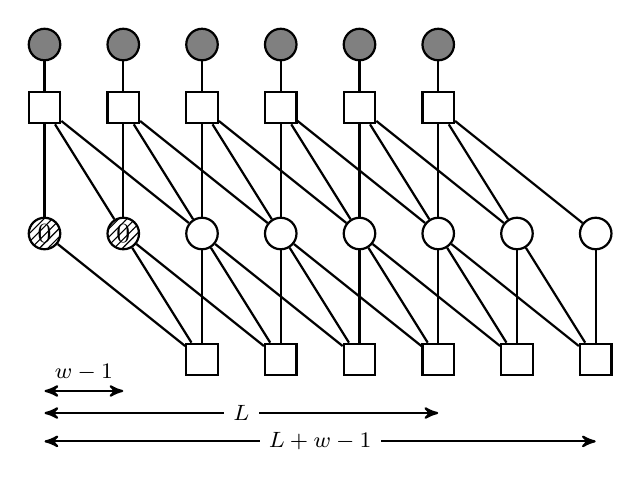
\begin{tikzpicture}
  [yscale=0.8,
  node distance = 12mm, draw=black, thick, >=stealth',
  bitnode/.style={circle, inner sep = 0pt, minimum size = 4mm, draw=black},
  bitnode2/.style={circle, inner sep = 0pt, minimum size = 4mm, draw=black, fill=gray},
  checknode/.style={rectangle, inner sep = 0pt, minimum size = 4mm, draw=black},
  ]

  \foreach \x in {1,...,6} {
    \node[bitnode2] (bu\x) at (\x,3) {};
  }

  \foreach \x in {1,...,6} {
    \node[checknode] (cu\x) at (\x,2) {};
  }

  \foreach \x in {1,2} {
    \node[bitnode,pattern=north east lines] (b\x) at (\x,0) {$0$};
  }

  \foreach \x in {3,...,8} {
    \node[bitnode] (b\x) at (\x,0) {};
  }

  \foreach \x in {1,...,6} {
    \node[checknode] (cl\x) at (\x+2,-2) {};
  }

  \foreach \x in {1,...,6} {
    \draw (bu\x) -- (cu\x);
  }

  \foreach \x/\y/\z in {1/2/3,2/3/4,3/4/5,4/5/6,5/6/7,6/7/8} {
    \draw (cu\x) -- (b\x);
    \draw (cu\x) -- (b\y);
    \draw (cu\x) -- (b\z);
  }

  \foreach \x/\y/\z in {1/2/3,2/3/4,3/4/5,4/5/6,5/6/7,6/7/8} {
    \draw (cl\x) -- (b\x);
    \draw (cl\x) -- (b\y);
    \draw (cl\x) -- (b\z);
  }

  \draw[<->] (1,-2.5) -- node[above]{\footnotesize{$w-1$}} (2,-2.5);
  \draw[<->] (1,-2.85) -- node[midway,fill=white]{\footnotesize{$L$}} (6,-2.85);
  \draw[<->] (1,-3.3) -- node[midway,fill=white]{\footnotesize{$L+w-1$}} (8,-3.3);

\end{tikzpicture}

%%% Local Variables: 
%%% mode: latex
%%% TeX-master: "../isit14"
%%% End: 

  \vspace{-2.5mm}
  \caption{Illustration of edge connections in a spatially-coupled compound LDGM/LDPC code.
    LDPC bit-nodes in the first $w-1$ groups are set to $0$.
  }
  \label{figure:protograph_coupled_compound}
\end{figure}
For convenience, we assume regular degrees in both LDGM and LDPC components of the compound code.
The construction can be easily generalized to irregular degrees.
Suppose $d_c$ and $d_v$ denote the degrees of the check- and bit-nodes, respectively, in the LDGM component.
Similarly, define $d'_v$ and $d'_c$ for the LDPC component.
See Fig.~\ref{figure:tanner_graph_compound_code} for an illustration.
Consider $L+w-1$ groups of LDPC bit-nodes at positions $\mathcal{N}_v=\{1,2,\ldots,L+w-1\}$, $L$ groups of LDGM check-nodes at positions $\mathcal{N}_c=\{1,\ldots,L\}$, $L$ groups of LDPC check-nodes at positions $\mathcal{N}'_c=\{w,2,\ldots,L+w-1\}$.
See Fig.~\ref{figure:protograph_coupled_compound}.

Choose $N$ large enough so that $N d_v/d_c, N d_v /w$, $N d'_v/d'_c, N d_v'/w \in \mathbb{N}$.
We first show the coupling structure in the LDGM part.
At each position $i \in \mathcal{N}_v$, place $N$ LDPC bit-nodes each with $d_v$ edge sockets.
Similarly, at each position $j \in \mathcal{N}_c$, place $N d_v/d_c$ LDGM check-nodes each with $d_c$ edge sockets.
At each bit- and check-node group, partition the $N d_v$ edge sockets into $w$ groups using a uniform random permutation, and denote these partitions, respectively, by $\mathcal{N}_{i,k}^v$, $\mathcal{N}^c_{j,k}$ where $1 \leq i \leq L+w-1$, $1 \leq j \leq L$, $1 \leq k \leq w$.
The coupled LDGM component is constructed by connecting the sockets in $\mathcal{N}^c_{j,k}$ to sockets in $\mathcal{N}^v_{j+k-1,k}$.
The coupling structure in the LDPC part can be constructed similarly.
These connections are depicted in Fig.~\ref{figure:protograph_coupled_compound} for $L=6$ and $w=3$.

We note that such a construction leaves some edge sockets of the LDPC bit-nodes at the boundary unconnected.
We also shorten the LDPC bit-nodes in the first $w-1$ groups to $0$.
This shortening and the unconnected edge sockets at the boundary are necessary for the spatial-coupling phenomenon to take effect \cite{Kudekar-it11}.
It is implicit that the LDPC check-nodes at each position in $\mathcal{N}'_c$ are partitioned into two groups $\mathcal{P}_1$ and $\mathcal{P}_2$ so as to have the desired design rate.
To avoid small error floors when decoding, each LDPC bit-node should have some connections to the checks in $\mathcal{P}_2$.
The characterization of the codebooks $\mathcal{SC}$, $\mathcal{SC}(s^k)$, $\mathcal{SC}'$, $\mathcal{SC}'(s^k)$ follows implicitly.

\subsection{Message-Passing Algorithms for Encoding}
\begin{algorithm}[!t]
\begin{algorithmic}
  \caption{Belief-Propagation Guided Decimation}
  \label{algorithm:bpgd}
  \REQUIRE{Sequence $x^n \in \{0,1\}^n$ to encode, parameters ($T$, $\beta$), graph $G(V,U,C)$.}
  \STATE Set $m_{i \to a}\!=\!\wh{m}_{a \to i}\!=\!0$ for $i \in V \cup U$, $a \in C$ and $(i,a) \in G$.
  \STATE Initialize $V_{\mathrm{dec}}$ to be LDPC bit-nodes in first $w-1$ sections.
  \WHILE{$V_{\mathrm{dec}} \neq V$}
    \FOR {$t=1$ to $T$}
      \STATE $m_{i \to a} = (-1)^{x_i} \tanh(\beta)$ for $i \in U$ and $a \in C$.
      \STATE $m_{i \to a} = (-1)^{u_i} \cdotp \infty$ for $i \in V_{\mathrm{dec}}$ and $a \in C$.
      \STATE $m_{i \to a} = \sum\limits_{b \in \partial i \setminus \{a\}} \wh{m}_{b \to i}$ for $i \in V \setminus V_{\mathrm{dec}}$ and $a \in C$.
      \STATE $\wh{m}_{a \to i} = \tanh^{-1} \prod\limits_{j \in \partial a \setminus \{ i \} } \tanh m_{j \to a}$ for $i \in V \setminus V_{\mathrm{dec}}$ and $a \in C$.
    \ENDFOR
    \STATE Evaluate $m_{i}=\sum_{a \in \partial i} \wh{m}_{a \to i} $ for all $i \in V\setminus V_{\mathrm{dec}}$.
    \STATE Set $B$ to be max. of $|m_i|$ when $i$ varies over left-most $w$ sections of $V \setminus V_{\mathrm{dec}}$; denote the resulting bit-node by $i^*$.
    \IF{$B=0$}
      \STATE Pick a bit-node $i^*$ uniformly in left-most $w$ sections of $V \setminus V_{\mathrm{dec}}$ and set $u_{i^*}$ to be $0$ or $1$ uniformly randomly.
    \ELSE
      \STATE Set $u_{i^*}$ to $0$ or $1$ with prob. $\frac{1+\tanh m_{i^*}}{2}$ or $\frac{1-\tanh m_{i^*}}{2}$.
    \ENDIF
    \STATE Set $V_{\mathrm{dec}} = V_{\mathrm{dec}} \cup \{i^*\}$.
  \ENDWHILE
  \STATE If $\{u_{i}\}$ fail to satisfy LDPC checks, then \textbf{re-encode}.
\end{algorithmic}
\end{algorithm}

Message-passing algorithms for channel coding are now a standard part of the coding theory literature.
We refer the reader to \cite{RU-2008} for their description.
It has been recently shown \cite{Obata-isit13}, \cite{Sakaniwa-arxiv11} that SC compound LDGM/LDPC codes are good for channel coding under message-passing.
As such, $\mathcal{SC}$, $\mathcal{SC}(s^k)$, $\mathcal{SC}'(s^k)$ are good for channel coding under message-passing.
In the following, we focus exclusively on the message-passing algorithm for rate distortion.
In particular, we describe a variation of the so-called BPGD algorithm \cite{Aref-arxiv13}, \cite{Aref-isit12}.

Consider an instance of the spatially-coupled compound LDGM/LDPC described above.
Denote its Tanner graph by $G(V,U,C)$, where $V$ denotes the LDPC bit-nodes, $U$ denotes the LDGM bit-nodes, $C$ denotes the check-nodes (both LDGM and LDPC).
Place a sequence $x^n \in \{0,1\}^n$ at the top of LDGM bit-nodes as in Fig.~\ref{figure:tanner_graph_compound_code}.
The message-passing rules here are same as in the channel coding setup by assuming that $x_i$ have come through a BSC channel (parameterized by $\beta$).
However, every $T$ iterations, an LDPC bit-node is decimated (shortened based on the current LLR).
This encoding procedure for the codebook $\mathcal{C}(s^k)$ is described in Algorithm \ref{algorithm:bpgd} assuming $s^k = 0^k$.
For $s^k \neq 0^k$, the update for each check node in $\mathcal{P}_1$ is modified to include the appropriate $s_k$ hard-decision message.
Also, the decimated sequence $u^n$ may not satisfy all the LDPC check constraints.
In this case, successive encoding attempts often result in a valid codeword due to the randomization in Algorithm \ref{algorithm:bpgd}.
In practice, we found that removing double edges and 4-cycles from the code essentially eliminated this problem at moderate block lengths.
For example, see the results in Table \ref{table:succ_enc}.

One variation in Algorithm \ref{algorithm:bpgd} from \cite{Aref-arxiv13} is the choice of the LDPC bit-node for decimation.
In \cite{Aref-arxiv13}, bit-node with maximum bias over entire graph is selected, but we restrict the search for maximum biased bit to only left-most $w$ sections of the bits that are not already decimated.
We observed that this change increases the chances of encoding to a valid codeword.
\begin{remark}
  The BPGD algorithm, when applied to the \emph{uncoupled} compound LDGM/LDPC code, always failed to satisfy the LDPC check constraints and the spatial-coupling structure is required to overcome this problem.
  Thus, spatial coupling in compound codes not only helps to reduce the distortion, but allows the BPGD algorithm to encode to a valid codeword.
\end{remark}
It is also possible to create a coupling structure in a circular fashion and decimate the bit-nodes in a fixed section as done in \cite{Aref-isit12}.
However, this leads to a \emph{wave} of decimations from both ends and will result in a failure to encode to a codeword, as the constraints imposed by the LDPC check-nodes are unlikely to match when the two waves meet.
From a physics point of view, this is akin to growing a crystal on a torus from a single seed.
When the two growth interfaces meet, they are very unlikely to mesh nicely and form a pure crystal.

%%% Local Variables: 
%%% mode: latex
%%% TeX-master: "isit14"
%%% End: 


\vspace{-0.0mm}
\section{Numerical Results}
\label{section:numerical_results}
Table \ref{table:succ_enc} shows the number of attempts required to encode $50$ source sequences in $\mathcal{C}(s^k)$, with $s^k=0^k$, over different block lengths. 
For example, at a block length of $9000$, $21$ sequences encoded in the first attempt and $9$ sequences did not encode in four attempts.
Without removing $4$-cycles, only $5$ sequences encoded at first and $35$ failed after 4 attempts.
%the number of attempts for the same parameters are $5/3/5/2/35$.
At a block length of $81000$, all $50$ sequences encoded in the first attempt.

Tables \ref{table:wyner_ziv} and \ref{table:gelfand_pinsker} provide the simulation results with SC compound codes with message-passing algorithms.
In the LDGM part of the code, $1\%$ of the check-nodes have degree 1.
This is to ensure that the decoding gets started for the channel coding problem.
Encoding for the WZ problem is relatively easy, since this is performed using the codebook $\mathcal{SC}'$, which does not have LDPC check constraints.
The optimal thresholds are calculated based on the rate of the code.
For example, if a code of rate $R$ is used to encode a $\mathsf{Ber}(\tfrac{1}{2})$, then $D_{*}=h^{-1}(1-R)$.
The reported distortion and the optimal thresholds correspond to the saturated section of the SC system uneffected by the boundary condition.

For the GP problem, half of all the LDPC check-nodes are chosen randomly to carry message bits, except in the $w-1$ sections at the boundary where no message bits are placed.
Since the bit-nodes in the left-most $w-1$ sections are initialized to $0$, the LDPC check nodes cannot carry any messages in the left-most $w-1$ sections.
Also, since the channel code for the GP problem uses fewer parity checks for the right boundary LDPC bit-nodes, there is a small error floor if we place message bits in the right-most $w-1$ sections.
To avoid this floor, we do not place message bits in these sections and instead incur a small rate loss.

%\vspace{-0.2cm}
\begin{table}[thb]
\begin{center}
\caption{No. of attempts for succ. encoding for $50$ codewords. 
  $(d_v,d_c,d'_v,d'_c)=(6,3,3,6)$, $(L,w)=(15,3)$, $(\beta,T)=(0.65,10)$.}
\label{table:succ_enc}
\vspace{-1mm}
\begin{tabular}{|c|c|c|}
\hline
Block length ($n$) & 4-cycles & $1/2/3/4/\geq 5$  \\
\hline
$9000$ & yes & $5/3/5/2/35$ \\
$9000$ & no & $21/12/5/3/9$ \\
$27000$ & no & $35/15/0/0/0$ \\
$45000$ & no & $40/9/0/0/1$ \\
$63000$ & no & $44/6/0/0/0$ \\
$81000$ & no & $50/0/0/0/0$\\ 
\hline  
\end{tabular}
\end{center}
\vspace{-0.65cm}
\end{table}

\begin{table}[thb]
\begin{center}
\caption{Thresholds for Wyner-Ziv problem with $(n\approx 140000,\beta=1.04,T=10)$.}
\label{table:wyner_ziv}
\vspace{-1mm}
\begin{tabular}{|p{0.8cm}|p{0.8cm}|p{0.7cm}|p{1.6cm}|p{1.65cm}|}
\hline
LDGM & LDPC & $(L,w)$ & $(D_{*},\delta_{*})$ & $(D,\delta)$ \\
$(d_v,d_c)$ & $(d'_v,d'_c)$ &  &  & \\
\hline
$(6,3)$ & (3,6) & (20,4)  & (0.111,0.134)  & (0.1174,0.122) \\
$(8,4)$ & (3,6) & (20,4)  & (0.111,0.134)  & (0.1149,0.120) \\
$(10,5)$ & (3,6) & (20,4)  & (0.111,0.134)  & (0.1139,0.122) \\
\hline  
\end{tabular}
\end{center}
\vspace{-0.65cm}
\end{table}

\begin{table}[thb]
\begin{center}
\caption{Thresholds for Gelfand-Pinsker problem with $(n\approx 140000,\beta=0.65,T=10)$.} 
\label{table:gelfand_pinsker}
\vspace{-1mm}
\begin{tabular}{|p{1.4cm}|p{0.8cm}|p{0.8cm}|p{1.4cm}|p{1.4cm}|}
\hline
LDGM & LDPC & $(L,w)$ & $(p_{*},\delta_{*})$ & $(p,\delta)$ \\
$(d_v,d_c)$ & $(d'_v,d'_c)$ &  &  & \\
\hline
$(6,3)$ & (3,6) & (20,4)  & (0.215,0.157)  & (0.220,0.152) \\
$(8,4)$ & (3,6) & (20,4)  & (0.215,0.157)  & (0.223,0.151) \\
$(10,5)$ & (3,6) & (20,4)  & (0.215,0.157)  & (0.220,0.151) \\
\hline
\end{tabular}
\end{center}
\vspace{-0.5cm}
\end{table}

%%% Local Variables: 
%%% mode: latex
%%% TeX-master: "isit14"
%%% End: 


\section{Conclusion}
We have considered SC compound LDGM/LDPC codes that achieve the rate regions of the WZ and GP side-information problems.
The decoding and encoding is based on message-passing algorithms.
The encoding is performed using BPGD algorithm.
For the WZ problem, LDGM codes were sufficient for the encoding to achieve the entire rate region.
For the GP problem, we require compound codes and the encoding here is more complicated since the LDPC bit-nodes need to satisfy additional constraints.
The structure enforced by spatial-coupling seems to be crucial for the BPGD algorithm to encode to a codeword in compound codes.
Numerical evidence is provided that shows that the SC compound codes can approach the desired rate regions.

\vspace{-0.0mm}
\bibliographystyle{ieeetr}
\bibliography{WCLabrv,WCLbib,WCLnewbib}

\end{document}
